\label{app:nas}
\section{Personalized Federated Neural Architecture Search}
\label{c4-sec:method}
Our method, $\textsc{FedPNAS}$, adopts the same over-parameterized architecture space as suggested by~\citet{hu2020}. Unlike~\citep{hu2020}, which lacks the ability to customize architectures for individual tasks, our method achieves architecture personalization via factorizing the architecture space into: (1)~a base component that is shared among all client models; and (2)~a task-specific component, which personalizes across clients to best solve their respective tasks (Section~\ref{c4-subsec:archspace}). We learn the operator mixing weights $\bar{m}(e)$ for all edges, which induce the joint distribution over all edge operators over two phases. 

In the \emph{federated} phase of \textsc{FedPNAS}, a common overall architecture is learned such that all task-specific architectures can be quickly and optimally derived from it with minimal fine-tuning efforts. This learning objective is achieved by extending the MAML meta learning algorithm proposed by~\citet{Finn17}. (Section~\ref{c4-subsec:objective}). Subsequently, in the \emph{adaptation} phase of \textsc{FedPNAS}, each client separately performs local update of its task-specific component using private data. Unlike other meta learning objectives~\citep{Finn17}, which only focus on adapting the weights of a single architecture, this adaptation step will result in diverging personalized architectures that are optimal for their respective tasks. The remainder of this section describes these contributions in details.


\subsection{Cell-based Architecture Space}
\label{c4-subsec:archspace}
Similar to~\citet{hu2020}, we express the over-parameterized architecture $\mathcal{G_O}$ as a stack of modular cells, i.e., $\mathcal{G}_0 = \bigcup_{t=1}^C \mathcal{G}_t$, where $C$ is the total number of cells and each cell $\mathcal{G}_t$ denotes a compact space of architecture constructed from the operator list $\mathcal{O}$. To obtain an architecture from $\mathcal{G_O}$, we first distill an architecture module $G_t = (V_t, E_t)$ from each cell by selecting a subset of edges in $\mathcal{G}_t$. The propagation path of the input vector across these modules is then heuristically chosen and specified by a cell-level DAG. For example, a simple linear propagation scheme can be written as $G(\mathbf{x}) = G_C \circ G_{C-1} \dots \circ G_1(\mathbf{x})$, where $\mathbf{x}$ denotes an input vector and each $G_i$ is treated as a feature map.

The inner computation of each distilled module $G_t$ is similarly defined as in Section~\ref{c5:nas}. Given an input vector $\mathbf{x}$, we then sample an operator $o_e$ on each edge $e \equiv (v, v') \in E_t$ from the vocabulary $\mathcal{O} \triangleq \left[o_1, o_2 \dots o_D\right]$ using a parameterized categorical distribution $p^t_e$.~\citet{hu2020} assumes this edge sampling distribution is independent of the input $\mathbf{x}$ and any intermediate feature mapping of $\mathbf{x}$, hence does not make use of these context information in deciding the distilled architecture. In the context of \emph{horizontal} NAS, we instead argue that these information are valuable in guiding client-level architecture adaptations and consequently parameterize $p^t_e$ as conditional sampling distributions, which jointly model a hierarchical decision process (Section~\ref{c4-subsec:opsampler}). 

The feature aggregation scheme for any arbitrary node $v' \in V_t$ is then given as:
\begin{eqnarray}
z_{v'} &=& \sum_{e\equiv(v,v')}^{e \in E_t} \mathbb{E}_{r \sim p^t_e}\left[r^\top \xi(z_v)\right] \ \simeq \ \sum_{e\equiv(v,v')}^{e \in E_t} \sum_{i=1}^s r_{ei}^\top \ \xi(z_v) \ ,
\end{eqnarray}
where each $r_{ei}$ is a one-hot vector drawn from $p^t_e$ and $\xi(z_v) \triangleq \left[o_1(z_v), o_2(z_v) \dots o_D(z_v)\right]$ is the concatenation of all possible transformations of $z_v$ using the operators in $\mathcal{O}$. Even though the computation above requires sampling from a categorical distribution, it can be made differentiable with respect to the parameters of $p^t_{e}$ using the straight through Gumbel-softmax trick~\cite{jang2016}. %We will detail the learning of these parameters in Section~\ref{c4-subsec:opsampler} 

Unlike the original design, which assumes similar importance for every cell in the architecture stack, we opt to split our cell-based architecture into two component stacks with different roles to facilitate our personalized architecture search goal. Specifically, our search space contains: (a) a \emph{base stack} $\mathcal{G}_b = \{\mathcal{G}_b^1, \mathcal{G}_b^2 \dots \mathcal{G}_b^{C_b}\}$, which aims to capture a feature map that is universally useful to all tasks; and (b) a \emph{personalized stack} $\mathcal{G}_p = \{\mathcal{G}_p^1, \mathcal{G}_p^2 \dots \mathcal{G}_p^{C_p}\}$, which will be adapted using client data to capture task-specific features. Fig.~\ref{app-nas-fig:architecture} summarizes the relationship of these components. 

\begin{figure}[h]
\centering
\begin{tikzpicture}
\node[io] (x) {$x$};
\node[group, minimum height=2.5em, minimum width=3em, right=1.5em of x] (b1) {$G_b^1$};
\node[group, minimum height = 5em, minimum width = 19em, right = 0.5em of x] (basestack) {};
\node[group, minimum height=2.5em, minimum width=3em, right=1.5em of b1] (b2) {$G_b^2$};
\node[group, minimum height=2.5em, minimum width=3em, right=1.5em of b2] (bdots) {\dots};
\node[above=1.5em of bdots] (invi2) {};
\node[right=0.5em of invi2] (invi) {};
\node[group, minimum height=2.5em, minimum width=3em, right=1.5em of bdots] (bc) {$G_b^{C_b}$};
\node[io, below=4em of x] (psix) {$G(x)$};
\node[group, minimum height = 5em, minimum width = 19em, right = 0.5em of psix] (specstack) {};
\node[group, minimum height=2.5em, minimum width=3em, right=1.5em of psix] (pc) {$G_p^{C_p}$};
\node[group, minimum height=2.5em, minimum width=3em, right=1.5em of pc] (pdots) {\dots};
\node[group, minimum height=2.5em, minimum width=3em, right=1.5em of pdots] (p2) {$G_p^{2}$};
\node[group, minimum height=2.5em, minimum width=3em, right=1.5em of p2] (p1) {$G_p^{1}$};
%\node[group2, minimum height=4.5em, minimum width=20em, right=1.1em of x] (bstack) {};
%\node[group2, minimum height=4.5em, minimum width=20em, right=1.1em of psix] (pstack) {};
\draw[conn] (x)--(b1);
\draw[conn] (b1)--(b2);
\draw[conn] (b2)--(bdots);
\draw[conn] (bdots)--(bc);
\draw[->] (x.north) to [out=45,in=90] (b2.north) node[above left=3.5em]{\tiny{\textsc{conv 1x1}}};
\draw[->] (b1.north) to [out=45,in=90] (bdots.north) node[above left=3.5em]{\tiny{\textsc{conv 1x1}}};
\draw[dashed,->] (invi.east) to [out=0,in=90] (bc.north) node[above left=3.5em]{\tiny{\textsc{conv 1x1}}};
\draw[conn] (bc)--(p1);
\draw[conn] (p1)--(p2);
\draw[conn] (p2)--(pdots);
\draw[conn] (pdots)--(pc);
\draw[conn] (pc)--(psix);
\end{tikzpicture}
\caption{Feature mapping induced by the component stacks of our architecture space. Each cell in the base stack receives outputs from two previous cells, whereas each cell in the personalized stack receives outputs from only one previous cell.}
\label{app-nas-fig:architecture}
\end{figure}

\noindent Generally, we assume that the tasks are broadly related and diverge in finer details. Therefore, the base architecture stack is designed to be significantly more expressive than the personalized stack, via employing a larger operator vocabulary and a more sophisticated propagation scheme as shown in Fig.~\ref{c4-fig:architecture}. In addition, as we will subsequently discuss in Section~\ref{c4-subsec:objective}, our objective is formulated such that its gradient evaluation will require approximating the Hessian of the personalized component. As such, a minimally expressive personalized stack is also a practical design to lower the computational cost. 


\subsection{Personalized Federated Learning Objective}
\label{c4-subsec:objective}
In this section, we will now discuss the learning objective of \textsc{FedPNAS}, which enables the discovery of personalized architecture. Let $\theta = \{\theta_b, \theta_p\}$ respectively denote all trainable parameters of the two component stacks above. In particular, $\theta_b=\{W_b, \Pi_b\}$ contains the concatenated weights $W_b$ of all edge operators; and the concatenated parameters $\Pi_b = [\Pi^t_e]_{t\in [C_b], e\in E_t}$ of the joint edge sampling distribution. Likewise, $\theta_p=\{W_p, \Pi_p\}$ contains their counterparts in the personalized stack. Given $N$ local clients with tasks $\{\Omega_1, \Omega_2 \dots \Omega_N\}$, the straight-forward extension of FL objective to the NAS problem defined by this search space can be written as:
\begin{eqnarray}
\theta_{\ast} &=& \underset{\theta}{\mathrm{argmax}} \frac{1}{N} \sum_{i=1}^N F_{\Omega_i}(\theta)
\label{c4-eq:flobj}
\end{eqnarray}
\citet{McMahan17} proposes a privacy preserving approach to optimize this objective by alternating between two communication steps of the model parameters. At any iteration $t \geq 0$:
\begin{itemize}
    \item Each local client performs a local gradient step with its current parameter $\theta^{t}_i$ and sends the suggested update $\bar{\theta}^t_i = \theta^t_i + \lambda\nabla_{\theta} F_{\Omega_i}(\theta^t_i)$ to a central server.
    \item The central server then computes $\theta^{t}_{\textsc{server}} = \frac{1}{N}\sum_{i=1}^N \bar{\theta}^t_i$ and broadcasts the aggregated parameters $\theta^{t}_{\textsc{server}}$ to all clients.
    \item Each local client performs the update $\theta^{t+1}_i \leftarrow \theta^{t}_{\textsc{server}}$ and prepares for the $(t+1)^{\text{th}}$ communication round.
\end{itemize}
This FL scheme implies that all clients will follow the same architecture distribution after the last communication round, which is not necessarily optimal in a heterogeneous task setting. To address this, our framework instead adopts the MAML meta learning objective~\citep{Finn17}, which aims to find a favorable initialization of $\theta$ that yields maximum averaged performance \textit{given an expected adaptation step}. This is different from Eq.~\ref{c4-eq:flobj}, which does not directly optimize for this initialization, but approximates it using the instantaneous averaged performance. Explicitly, this is achieved by the following objective:
\begin{eqnarray}
\theta_\ast &=& \underset{\theta_b, \theta_p}{\argmax} \frac{1}{N} \sum_{i=1}^N F_{\Omega_i}\left(\theta_b, \theta_p + \textcolor{red}{\lambda \nabla_{\theta_p} F_{\Omega_i}(\theta_b, \theta_p)} \right) \ ,
\label{c4-eq:fedpnasobj}
\end{eqnarray}
in which the difference from Eq.~\eqref{c4-eq:flobj}, highlighted in red, models a gradient ascent update with step size $\lambda$ to the aggregated personalized parameters $\theta_p$, which is to be conducted by each client at the end of the federated phase. Intuitively, this gradient step acts as a regularization term which favors $\theta$ that are simultaneously close to all task-specific optima and yield the best averaged performance after the adaptation phase. 

We now derive the gradient of this objective and discuss a practical algorithm to perform its computation. First, we let $\tilde{\theta}^t \triangleq \left(\theta^t_b, \theta^t_p + \lambda \nabla_{{\theta}^t_p} F_{\Omega}(\theta^t_b, \theta^t_p)\right)$ denote the anticipated update of $\theta$ at time $t$ of some arbitrary client. Then, dropping the client index for clarity, we subsequently derive the gradient ascent update for each client pertaining to the above personalized FL objective:
\begin{eqnarray}
\bar{\theta}^t &=& \theta^t + \lambda \nabla_{\theta^t} F_{\Omega}\left(\tilde{\theta}^t\right)\nonumber \\
&=& \theta^t + \left(\lambda \nabla_{\theta^t}\tilde{\theta}^t \right)\left(\nabla_{\tilde \theta^t} F_{\Omega}(\tilde{\theta_t})\right) \nonumber \\
&=& \theta^t +
\left[
\begin{array}{cc}
     \lambda\mathbf{I} &  \lambda^2 \nabla_{\theta_b^t} \nabla_{\theta_p^t} F_{\Omega}(\theta^t_b, \theta^t_p)\\
     \mathbf{0} & \lambda^2 \nabla^2_{\theta_p^t} F_{\Omega}(\theta^t_b, \theta^t_p)
\end{array}
\right]
\left(\nabla_{\tilde \theta^t} F_{\Omega}(\tilde{\theta}^t)\right) \ ,
\label{c4-eq:fedpnasexactgrad}
\end{eqnarray}
where we applied chain rule in the second equality and subsequently expanded $\lambda \nabla_{\theta^t}\tilde{\theta}^t$ in the third equality. The second-order gradient terms $\nabla_{\theta_b^t} \nabla_{\theta_p^t} F_{\Omega}(\theta^t_b, \theta^t_p)$ and $\nabla^2_{\theta_p^t} F_{\Omega}(\theta^t_b, \theta^t_p)$, however, are expensive to evaluate exactly. In order to derive practical computations of these terms, we note that the first-order Taylor approximation of the Hessian $\nabla^2_{\theta_p^t} F_{\Omega}(\theta^t_b, \theta^t_p)$ can be written as:
\begin{eqnarray}
\hspace{-8mm}
\nabla^2_{\theta^t} F_{\Omega}(\theta^t_b, \theta^t_p) &=& 
\left[
\begin{array}{cc}
     \nabla^2_{\theta_b^t} F_{\Omega}(\theta^t_b, \theta^t_p) &   \nabla_{\theta_b^t} \nabla_{\theta_p^t} F_{\Omega}(\theta^t_b, \theta^t_p)\\
     \nabla_{\theta_p^t} \nabla_{\theta_b^t} F_{\Omega}(\theta^t_b, \theta^t_p) & \nabla^2_{\theta_p^t} F_{\Omega}(\theta^t_b, \theta^t_p)
\end{array}
\right] \nonumber \\
&\simeq&
\left[
\begin{array}{c}
     \nabla_{\theta_b^t} F_{\Omega}(\theta^t_b, \theta^t_p) \\  \nabla_{\theta_p^t} F_{\Omega}(\theta^t_b, \theta^t_p)
\end{array}
\right]
\left[
\begin{array}{c}
     \nabla_{\theta_b^t} F_{\Omega}(\theta^t_b, \theta^t_p) \\  \nabla_{\theta_p^t} F_{\Omega}(\theta^t_b, \theta^t_p)
\end{array}
\right]^\top \nonumber \\
&=& 
\left[
\begin{array}{cc}
     \nabla_{\theta^t_b} F_{\Omega}(\theta^t_b, \theta^t_p)\nabla^\top_{\theta^t_b} F_{\Omega}(\theta^t_b, \theta^t_p)&   \nabla_{\theta^t_b} F_{\Omega}(\theta^t_b, \theta^t_p)\nabla^\top_{\theta^t_p} F_{\Omega}(\theta^t_b, \theta^t_p)\\
     \nabla_{\theta^t_p} F_{\Omega}(\theta^t_b, \theta^t_p)\nabla^\top_{\theta^t_b} F_{\Omega}(\theta^t_b, \theta^t_p)& \nabla_{\theta^t_p} F_{\Omega}(\theta^t_b, \theta^t_p)\nabla^\top_{\theta^t_p} F_{\Omega}(\theta^t_b, \theta^t_p)
\end{array}
\right] \ .
\end{eqnarray}
Matching appropriate terms in the above derivation then implies the following approximations, which can be computed with a single forward-backward pass of the architecture:
\begin{eqnarray}
\nabla_{\theta_b^t} \nabla_{\theta_p^t} F_{\Omega}(\theta^t_b, \theta^t_p)
&\simeq& \nabla_{\theta^t_b} F_{\Omega}(\theta^t_b, \theta^t_p)\nabla^\top_{\theta^t_p} F_{\Omega}(\theta^t_b, \theta^t_p) \ ,
\\
\nabla^2_{\theta_p^t} F_{\Omega}(\theta^t_b, \theta^t_p) &\simeq& \nabla_{\theta^t_p} F_{\Omega}(\theta^t_b, \theta^t_p)\nabla^\top_{\theta^t_p} F_{\Omega}(\theta^t_b, \theta^t_p) \ .
\end{eqnarray}
Plugging this back to Eq.~\eqref{c4-eq:fedpnasexactgrad} gives:
\begin{eqnarray}
\bar{\theta}^t &\simeq& 
\theta^t + 
\left[
\begin{array}{cc}
     \lambda \mathbf{I} & \lambda^2 \nabla_{\theta^t_b} F_{\Omega}(\theta^t_b, \theta^t_p)\nabla^\top_{\theta^t_p} F_{\Omega}(\theta^t_b, \theta^t_p) \\
     \mathbf{0} & \lambda^2
     \nabla_{\theta^t_p} F_{\Omega}(\theta^t_b, \theta^t_p)\nabla^\top_{\theta^t_p} F_{\Omega}(\theta^t_b, \theta^t_p)
\end{array}
\right]
\left(\nabla_{\tilde \theta^t} F_{\Omega}(\tilde{\theta^t})\right) \ ,
\label{c4-eq:fedpnasapproxgrad}
\end{eqnarray}
where the term $\nabla_{\tilde \theta^t} F_{\Omega}(\tilde{\theta^t})$ requires another forward-backward pass to compute (i.e., $\tilde{\theta}^t$ is computed in the same pass with the two approximated gradient terms above). Overall, this results in a local update scheme which uses two forward-backward passes of the architecture per iteration:
\begin{itemize}
    \item Compute $F_{\Omega}(\theta^t)$ in the first forward pass.
    \item Perform backpropagation to obtain $\nabla_{\theta^t} F_{\Omega}(\theta^t) = \left[\nabla_{\theta^t_b} F_{\Omega}(\theta^t_b,\theta^t_p), \nabla_{\theta^t_p} F_{\Omega}(\theta^t_b,\theta^t_p)\right]$. 
    \item Compute  $\nabla_{\theta^t_b} F_{\Omega}(\theta^t_b, \theta^t_p)\nabla^\top_{\theta^t_p} F_{\Omega}(\theta^t_b, \theta^t_p)$ and  $\nabla_{\theta^t_p} F_{\Omega}(\theta^t_b, \theta^t_p)\nabla^\top_{\theta^t_p} F_{\Omega}(\theta^t_b, \theta^t_p)$.
    \item Compute $\tilde{\theta}^t = \left(\theta^t_b, \theta^t_p + \lambda \nabla^\top_{\theta^t_p} F_{\Omega}(\theta^t_b, \theta^t_p)\right)$.
    \item Compute $F_{\Omega}(\tilde{\theta}^t)$ in the second forward pass.
    \item Perform backpropagation to obtain $\nabla_{\tilde{\theta}^t} F_{\Omega}(\tilde{\theta}^t)$.
    \item Compute the update in Eq.~\eqref{c4-eq:fedpnasapproxgrad}.
\end{itemize}

\subsection{Context-Aware Operator Sampling}
\label{c4-subsec:opsampler}
Finally, this section describes the parameterization of the joint operator sampling distribution over the edges of $\mathcal{G}_O$. Let $O_G \triangleq \cup_{t\in[C]} O_{G_t}$ be the set of all selected edge operators in a distilled architecture $G$, where $O_{G_t} \triangleq \{o^t_e \in \mathcal{O}\}_{e\in E_t}$ in turn denotes the set of all selected edge operators in cell $G_t$ (i.e., in a single stack architecture).~\citet{hu2020} then assumes a fully factorizable sampling distribution:
\begin{eqnarray}
p(O_G) 
&=& \prod_{t\in[C]} p(O_{G_t}) 
\ = \ \prod_{t\in[C]} \prod_{e \in E_t} p^t_e(o^t_e; \Pi^t_e) \ , 
\end{eqnarray}
where $\Pi^t_e$ denotes the learnable parameters of the edge sampling distribution $p^t_e$ for every $t \in [C]$ and $e \in E_t$. This formulation, however, does not factor in the important context information carried by the input instance $\mathbf{x}$ and its subsequent embeddings as $\mathbf{x}$ propagates through $G$. While this approach might be sufficient when only one architecture needs to be distilled from $\mathcal{G_O}$, it is challenging to extend to the \emph{horizontal} NAS setting because every edge in the over-parameterized architecture $\mathcal{G_O}$ is required to maintain and optimize its own set of categorical distribution parameters. In the context of our \emph{horizontal} NAS problem, this means that the set of parameters that need to be personalized will also scale with the size of the architecture, hence posing both a computational and a convergence problem. 

To overcome this issue, we will instead look at the conditional sampling distribution $p(O_g \mid \mathbf{x})$ and subsequently model architecture distillation as a Markov chain decision process, where each cell in the architecture stack will sequentially determine its edge operators given the input feature it receives from previous cells. For simplicity, we give our factorization of $p(O_G \mid \mathbf{x})$ below as if the architecture contains a single stack of cells and uses a linear propagation scheme, but it would be trivial to extend this formulation to any other propagation scheme:
\begin{eqnarray}
p(O_G \mid \mathbf{x}) &=& p(O_{G_1} \mid \mathbf{x}) \prod_{t=2}^C p(O_{G_t} \mid O_{G_{t-1}}, \mathbf{x}) \nonumber \\
%&\simeq& \prod_{t=1}^C p\left(O_{G_t} \mid z_{v^t_0}\right) \nonumber \\
&\simeq& \prod_{t=1}^C \prod_{e\equiv(v,v')}^{e \in E_t} p^t_e\left(o^t_{v,v'} \mid z_{v}\right) 
\end{eqnarray}
where $z_{v}$ denotes the feature vector at an arbitrary node $v$ in $G$ and in the factorization above, we have also assumed that $z_{v}$ acts as the sufficient statistics of the random variable $o^t_{v,v'}$.

The advantage of this formulation is two-fold. First, it provides a natural mechanism to incorporate context information into the edge selection process, thus allowing $\textsc{FedPNAS}$ to efficiently memorize architecture distillation patterns across clients. Second, the above factorization of $p(O_G \mid \mathbf {x})$ as a product of edge-wise conditional probabilities further reveals a compact representation of all sampling parameters using a single neural network $\psi$, which reduces the number of parameters that require fine-tuning in the local adaptation phase. That is, for any edge $e \equiv (v, v') \in E_t$, its context-aware operator distribution conditioned on $z_v$ is given as $p^t_e(o^t_{v,v'} \mid z_{v}) \triangleq \mathrm{Cat}\left(D, \psi\left(z_{v}\right)\right)$, where $D$ denotes the number of operators in $\mathcal{O}$ and the neural network $\psi$ maps the $z_{v}$ to the event probabilities of a categorical distribution.

\section{Experiments}
\label{c4-sec:exp}
This section describes our experiments to showcase the performance of $\textsc{FedPNAS}$ compared to other NAS and FL benchmarks. Our empirical studies are conducted on two image recognition datasets: (a) the CIFAR-10 dataset~\citep{cifar10} which aims to predict image labels from $10$ classes given a train/test set of $50000/10000$ colour images of dimension $32 \times 32$ pixels; and (b) the MNIST dataset~\citep{lecun2010mnist} which aims to predict handwritten digits (i.e. $0$ to $9$) given a train/test set of $60000/10000$ grayscale images of dimension $28 \times 28$ pixels. Our search space entails $2^{40}$ possible architectures, which is detailed in Appendix D. We compare two variants of our framework, \textsc{CA-FedPNAS} (with context-aware operation sampler) and \textsc{FedPNAS} (without the operation sampler), against:
(a) \textsc{FedAveraging} of a fixed architecture to justify the need for NAS in FL; (b) \textsc{FedDSNAS} - which trivially extends DSNAS to the FL setting (Eq.~\eqref{c4-eq:flobj}); and finally (c) \textsc{CA-FedDSNAS}, which extends \textsc{FedDSNAS} with our context-aware sampler.

\subsection{Heterogeneous predictive tasks} 
We first design a control experiment to test our framework on heterogeneous tasks and demonstrate the necessity of architecture personalization. To simulate this scenario, we first distribute the data i.i.d across clients (10000/2000 and 12000/2000 training/test images per client for CIFAR-10 and MNIST datasets respectively). Then, we independently apply a different transformation to each partitioned dataset. Input images within the same train/test set is subject to the same transformation. In both our experiments, the client datasets are subjected to rotations of $-30^{\circ}, -15^{\circ}, 0^{\circ}, 15^{\circ}$ and $30^{\circ}$ respectively. Fig.~\ref{fig4} below shows the performance of all the methods in comparison, plotted against number of search epochs and averaged over the above rotated variants of CIFAR-10 and MNIST datasets.

\begin{figure}[h]
\begin{tabular}{ccc}
\hspace{-6mm}
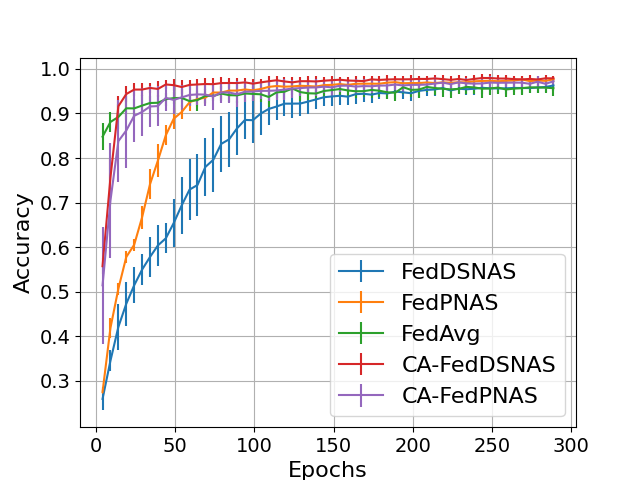
\includegraphics[width=0.33\columnwidth]{nas_plots/exp4.png} & 
\hspace{-6mm}
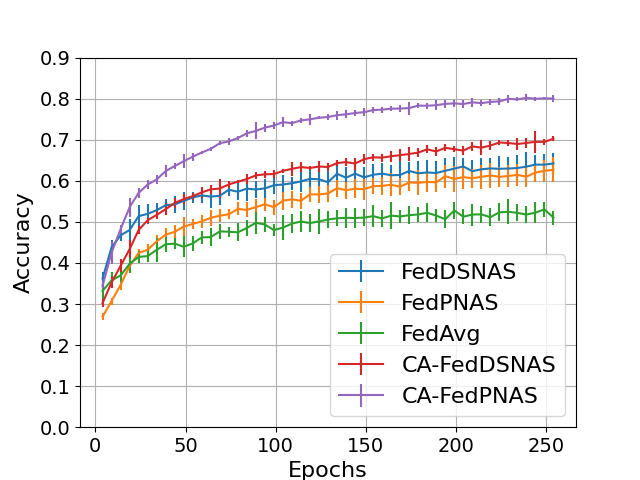
\includegraphics[width=0.33\columnwidth]{nas_plots/exp3.png} & 
\hspace{-6mm}
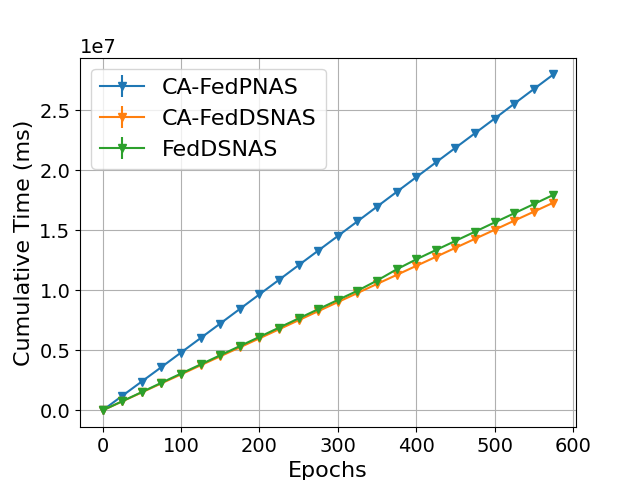
\includegraphics[width=0.33\columnwidth]{nas_plots/exp8.png} \\
\hspace{-6mm} (a) & 
\hspace{-6mm} (b) & 
\hspace{-6mm} (c)
\end{tabular}    
\caption{Plotting average classification accuracy of various methods against no. training epochs on heterogeneous tasks derived from (a) MNIST and (b) CIFAR-10 dataset. Figure (c) compares cumulative running time of various methods against no. training epochs on the CIFAR-10 dataset.}
\label{fig4}
\end{figure} 
On the MNIST dataset (Fig.~\ref{fig4}b), all methods converge to a similar performance. Among the NAS benchmarks, \textsc{FedPNAS} and \textsc{FedDSNAS} both converge slower than \textsc{FedAvg} and start off with worse performance in early iterations. This is expected since \textsc{FedAvg} does not have to search for the architecture and it is likely that the default architecture is sufficient for the MNIST task. On the other hand, we observe that both \textsc{CA-FedPNAS} and \textsc{CA-FedDSNAS} converge much faster than their counterparts without the context-aware operation sampler component. This shows that making use of contextual information helps to quickly locate regions of high-performing architectures, especially on similar inputs.

On the CIFAR-10 dataset  (Fig.~\ref{fig4}a), we instead observe significant gaps between the worst performing \textsc{FedAvg} and other NAS methods. This is likely because the default architecture does not have sufficient learning capability, which confirms the need for customizing solutions. Among the NAS benchmarks, we again observe that both \textsc{CA-FedPNAS} and \textsc{CA-FedDSNAS} outperform their counterparts without our operation sampler, which confirms the intuition above. Most remarkably, our proposed framework \textsc{CA-FedPNAS} achieves the best performance (0.8) and significantly outperformed both variants of federated \textsc{DSNAS} (0.71 for \textsc{CA-FedDSNAS} and 0.63 for \textsc{FedDSNAS}). 

Lastly, Fig.~\ref{fig4}c shows the runtime comparison between three methods on the CIFAR-10 experiment. In terms of sampling time, we observe that there is negligible overhead incurred by using our context-aware sampler (\textsc{CA-FedDSNAS} vs. \textsc{FedDSNAS}). 
The time incurred by our update (\textsc{CA-FedPNAS}) scales by a constant factor compared to \textsc{CA-FedDSNAS} since we use exactly one extra forward-backward pass per update. 

\begin{table}
	\centering
	\begin{sc}
		\begin{tabular}{|c|c|c|c|}
		\hline
		\multirow{2}{*}{Heterogeneity} & Task & \multirow{2}{*}{FedDSNAS} &  \multirow{2}{*}{CA-FedPNAS}\\
		& Description & & \\
		\hline
		\multirow{5}{*}{Low} & Rotate -30 & 0.947 & \textbf{0.978} \\
		\cline{2-4}
		& Rotate -15 & 0.973 & \textbf{0.976} \\
		\cline{2-4}
		& Vanilla & \textbf{0.988} & 0.985 \\
		\cline{2-4}
		& Rotate 15 & 0.986 & \textbf{0.987} \\
		\cline{2-4}
		& Rotate 30 & 0.972 & \textbf{0.981} \\
		\hline
		\multirow{5}{*}{High} & HueJitter -0.5 & 0.966 & \textbf{0.978} \\
		\cline{2-4}
		& HueJitter 0.5 & 0.967 & \textbf{0.972} \\
		\cline{2-4}
		& Vanilla & 0.988 & \textbf{0.989} \\
		\cline{2-4}
		& Rotate -90 & 0.892 & \textbf{0.932} \\
		\cline{2-4}
		& Rotate 90 & 0.866 & \textbf{0.932} \\
		\hline
	\end{tabular}
	\end{sc}
	\caption{Predictive accuracy of  \textsc{CA-FedPNAS} \textsc{FedDSNAS} on tasks with varying heterogeneity levels. \textsc{Rotate X}  denotes a rotation transformation of \textsc{X}$^{\circ}$ on client data; \textsc{Vanilla} denotes the original MNIST images; and \textsc{HueJitter X} denotes a hue jitter transformation of training images by a factor of \textsc{X}. The best performance in each row is in bold font.}
	\label{c4-table:1}
\end{table}

\subsection{Tasks with varying heterogeneity levels}
We expand the above study by subsequently investigating the respective performances of \textsc{CA-FedPNAS} and \textsc{FedDSNAS} on tasks with varying levels of heterogeneity. At low levels of heterogeneity, we deploy these methods on 5 sets of slightly rotated MNIST images. At high levels of heterogeneity, we employ a more diverse set of transformations on MNIST images, such as hue jitter and large angle rotations of $90^{\circ}$ and $-90^{\circ}$. Table~\ref{c4-table:1} shows the respective result of each task from these two settings. We observe that our method $\textsc{CA-FedPNAS}$ achieves better performance on most tasks and the performance gaps on tasks with higher heterogeneity are more pronounced (i.e., up to $7\%$ improvement on \textsc{Rotate 90} task). This clearly shows the importance of architecture personalization when the training tasks are significantly different and justifies our research goal.

\subsection{Knowledge transfer to completely new tasks} 
Finally, we conduct an ablation study to assess the quality of the \emph{pre-adaptation} architecture distributions respectively discovered by \textsc{CA-FedPNAS} and  \textsc{FedDSNAS}. In particular, we will leverage these learned distributions, which supposedly capture the broad commonalities of the task distribution, to generalize to completely unseen tasks (i.e., tasks that do not participate in the federated learning phase). To simulate this scenario, we train both methods on five clients whose local data consist of 12000 rotated CIFAR-10 images (i.e., in the range of $\pm 30^{\circ}$), similar to the setting of the first experiment. During the evaluation phase, however, we supply each local client with 2000 test images subjected to related but completely unseen transformations (i.e., $90^{\circ}$ and $-90^{\circ}$ rotations). 

\begin{table}[h]
	\centering
	\begin{sc}
		\begin{tabular}{|c|c|c|c|c|}
		\hline
		Unseen Task &  \multirow{2}{*}{FedDSNAS} & \multirow{2}{*}{CA-FedPNAS} & FedDSNAS & CA-FedPNAS \\
		Description & & & (Retrained) & (Retrained) \\
		\hline
		Rotate -90 & 0.545 $\pm$ 0.04 & 0.578 $\pm$ 0.09 & 0.699 $\pm$ 0.12 & \textbf{0.734 $\pm$ 0.17} \\
		\hline
		Rotate 90 & 0.553 $\pm$ 0.12 & 0.569 $\pm$ 0.06 & 0.673 $\pm$ 0.13 & \textbf{0.727 $\pm$ 0.22} \\
		\hline
		\end{tabular}
	\end{sc}
	\caption{Predictive accuracy (averaged over 5 clients) and standard deviation of \textsc{CA-FedPNAS} and \textsc{FedDSNAS} on two unseen tasks (CIFAR-10).}
	\label{c4-table:2}
\end{table}

\noindent We summarize our results in Table~\ref{c4-table:2} above. First, we measure the performance of \textsc{CA-FedPNAS} and \textsc{FedDSNAS} without any weight retraining. When received no additional information from the unseen tasks, both methods perform poorly as expected. While $\textsc{CA-FedPNAS}$ achieves better predictive accuracy, the performance gap in this scenario is negligible. To provide additional clues for adaptation, albeit minimal, we retrain the weights of each local model with 200  images that are rotated according to their respective unseen task description. With only 100 retraining iterations on limited data, \textsc{CA-FedPSNAS} already outperforms \textsc{FedDSNAS} (5\% and 8\% improvement respectively on two unseen tasks). This implies that \textsc{CA-FedPNAS} has captured more accurately the broad similarity of the task spectrum and requires minimal additional information to successfully adapt to unseen tasks.